\chapter*{\label{ref-010}Hilversum, Den Haag, Dordrecht: kinderen}

Nadat ik getrouwd was moest ik dat doorgeven aan het kantoor van de Kinderbescherming in Den Haag en kreeg ik dus (!) mijn ontslag. Maar ik mocht toch wel doorwerken en werd voortaan gedetacheerd als er ergens te weinig mensen waren. Ik wilde wel graag doorwerken want Joop voer dus ik was best veel alleen.

Ik vond het leuk om te trouwen maar ik kon het niet uitstaan dat ik stoppen moest met werken. Ik vond het verschrikkelijk dat ik mijn eigen geld niet meer kon verdienen toen de kinderen werden geboren, ik vond dat ik zelf voor een inkomen moest zorgen. Maar dat kon niet, het ging anders. Ik was 29 jaar toen ik ging trouwen.
 
Toen de kinderen groot waren heb ik nog wel eens overwogen om weer aan het werk te gaan. Mij is toen verteld dat ik het waarschijnlijk niet leuk meer zou vinden omdat het gedrag van de kinderen heftiger was dan in de tijd dat ik nog werkte. Ik heb toen besloten om het niet te doen.

We hebben eerst ingewoond in Hilversum bij de moeder van een collega, mevrouw IJma. We hadden een eigen etage met een flinke kamer boven met een slaapkamer. Koken was een beetje primitief in een soort werkkast met een elektrisch pitje. Het was best wel leuk. Joop ging natuurlijk weer varen; nog wel korte reisjes van 2 tot 3 maanden. 

\begin{figure}[h]
    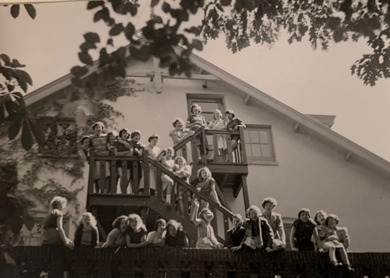
\includegraphics[width=\textwidth]{image43}
    \caption{Gedetacheerd in Den Dolder.}
\end{figure}

 Ik werkte onder andere bij een instelling voor kinderbescherming in Den Dolder en Hilversum voor iets oudere kinderen (14-17). Daar werkte ik als waarnemend directrice. Ik moest de werkzaamheden van iedereen inplannen en viel in op de groepen als het nodig was. Ik werd gedetacheerd naar diverse instellingen.

Na een tijdje gingen we verhuizen naar Den Haag. Via de zus van Joop konden we in het huis van hun buren terecht. Daar konden we een deel van onderhuren. Het was een ouder echtpaar en ze waren er vaak niet. En gelukkig waren ze reuze makkelijk. Zij hadden daar de voorkamer en wij de achterkamer met een klein slaapkamertje en een balkon. De woningnood was toen, zo vlak na de oorlog, nog erg groot. 



Toen we net getrouwd waren ging Joop weg op een ontzettende lange reis. Toen we net verloofd waren ging hij een jaar weg, maar toen werkte ik nog, dus was het gemis minder. 

Op een gegeven moment kwam er een beter ritme met kortere reizen. Vooral toen hij naar Zuid-Afrika ging, want dat waren zes weken. Maar ja, dat wilde iedereen wel natuurlijk, dus dat moesten ze een beetje verdelen. 

Nou ja, het gebeurt en de \'{e}\'{e}n kan er tegen en de ander niet. Als je niet z\'{o} bij moeder vandaan komt en dan trouwt met iemand die constant weg is gaat het beter. Als je je eigen werk hebt.

Ik raakte in Den Haag in verwachting en stopte met werken. Jacqueline is op 4 februari 1958 in het ziekenhuis geboren. Joop was net van een kustreis terug. Hij kwam thuis van een lange reis en moest daarna nog een kustreis en dat ging allemaal n\'{e}t! Jacqueline is in de Oranjekliniek in Den Haag geboren, want we woonden in. We hadden geen ruimte om thuis te bevallen.

\begin{figure}[h]
    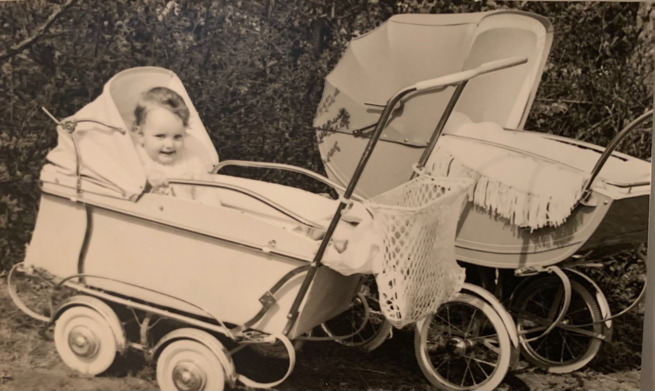
\includegraphics[width=\textwidth]{image47}
    \caption{In de kinderwagen.}
\end{figure}

Joop studeerde toen voor zijn tweede rang; hij moest daarvoor naar school in Amsterdam. Dat kwam wel even mooi uit. Ik moest wel wennen toen hij daarna weer weg ging en ik alles alleen moest doen.

\begin{figure}[h]
    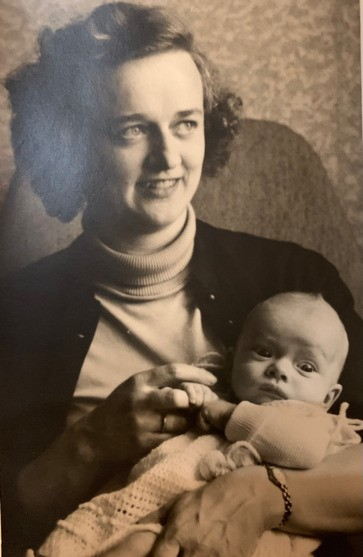
\includegraphics[width=0.9\textwidth]{image45}
    \caption{Jonge moeder.}
\end{figure}

\begin{figure}[h]
    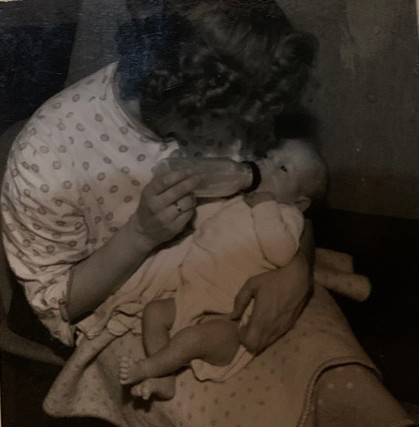
\includegraphics[width=\textwidth]{image44}
    \caption{Jacqueline krijgt te drinken.}
\end{figure}

We hebben dus nog een jaar ondergehuurd met een baby. Het was vooral gezellig met m’n schoonzus en zwager als buren. 

En we zaten vlak bij het Haagse bos. Ik ging vaak wandelen met Han, mijn schoonzus en onze baby’s. Ik had het er best naar mijn zin!

\begin{figure}[h]
    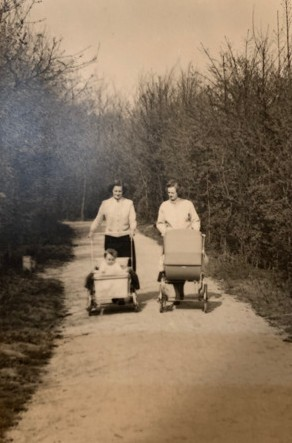
\includegraphics[width=.9\textwidth]{image46}
    \caption{Wandelen in het Haagse bos.}
\end{figure}

De maatschappij waar Joop werkte, de VNS, liet vervolgens in Dordrecht een appartementengebouw neerzetten voor zeevarenden. Daar kregen wij eindelijk ons eerste eigen huis! 

De hunkerbunker noemden de mannen dat gebouw. Want ja met al die vrouwen van zeevarenden daar...

Ik kon er wel tegen; ik zocht wat anders om me mee bezig te houden. Ik was gelukkig al jaren zelfstandig. Maar er waren ook vrouwen die er echt niet tegen konden. Dat was het laatste wat ik wou, dat mijn man met zijn werk moest stoppen omdat ik niet op mijn eigen benen zou kunnen staan. Maar ik had het af en toe ook wel moeilijk.

In de flat kreeg ik een leuke vriendin, Jannie Punt. Wij hebben ons hele leven contact gehouden. Maar nu we zo heel oud zijn wordt dat wat lastiger. Het waren verder beste mensen, maar daar ging ik niet mee om. Jannie Punt was degene waar ik het meeste contact mee had.

In Dordrecht is Yvonne geboren, op 20 april 1959, ruim een jaar na Jacqueline.

\begin{figure}[h]
    \begin{centering}
    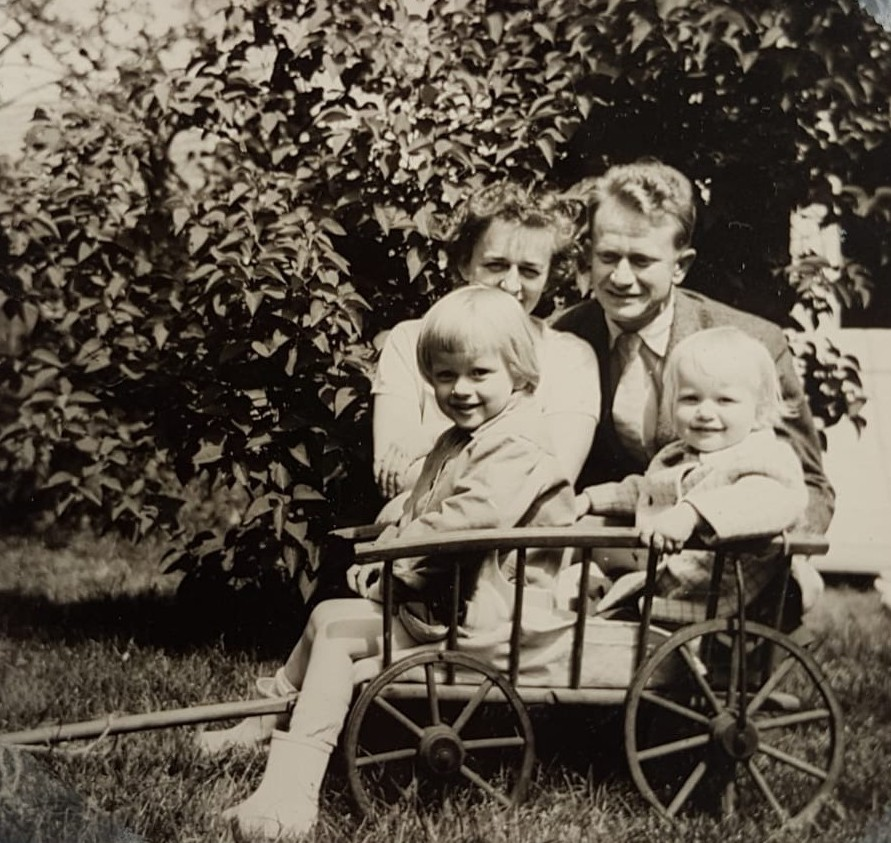
\includegraphics[width=\textwidth]{image49}
    \caption{Het hele gezin.}
    \end{centering}
\end{figure}

Een hele aardige dokter had ik toen. Hij was ook gewoon zorgzaam, zo van ‘die man zit op zee...’.

\begin{figure}[h]
    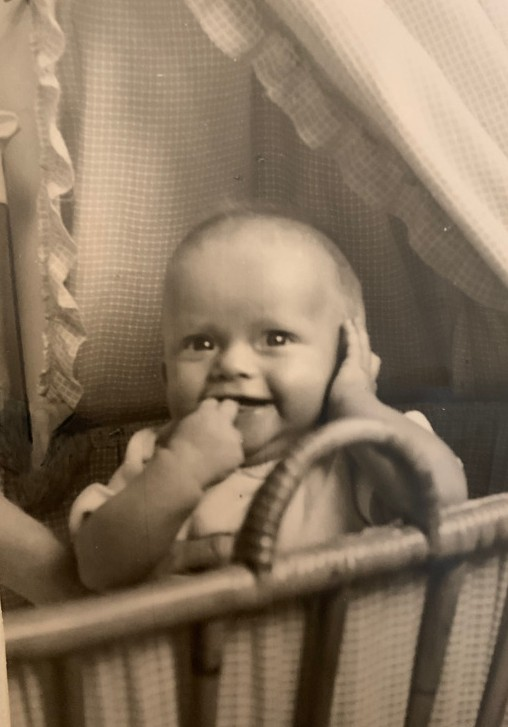
\includegraphics[width=.9\textwidth]{image48}
    \caption{Yvonne.}
\end{figure}

Joop was toen ook een periode wat langer thuis voor z’n eerste rang te halen; hij moest in Scheveningen naar de zeevaartschool. Dat was wel een hele leuke en gezellige periode! Hij had ook een vak in het Engels en dat deden we dan samen. 

De bevalling was ’s nachts al begonnen en ik dacht: Ik ga die dokter nog niet bellen, maar tegen 7 uur vond ik het wel tijd worden. Hij kwam ook snel en Yvonne werd thuis geboren. 

En het was hartstikke gezellig hoor, het thuis bevallen. Als het allemaal goed gaat, vind ik dat thuis veel leuker. En het waren geen zware bevallingen. Ik zei wel eens: ``Wat dat betreft kan ik er wel 12 op de wereld zetten.'' Jacqueline was net bij Jannie Punt gebracht en de melkboer kwam aan de deur en zei tegen Joop: ik hoor volgens mij al een baby huilen. Kortom een zeer snelle geboorte.

Ik kreeg Jacqueline en Yvonne snel achter elkaar. Toen wist ik wat ik moest doen. Ik vond het voor de kinderen leuk dat ze zo weinig scheelden.